\begin{figure}[H]
    \centering

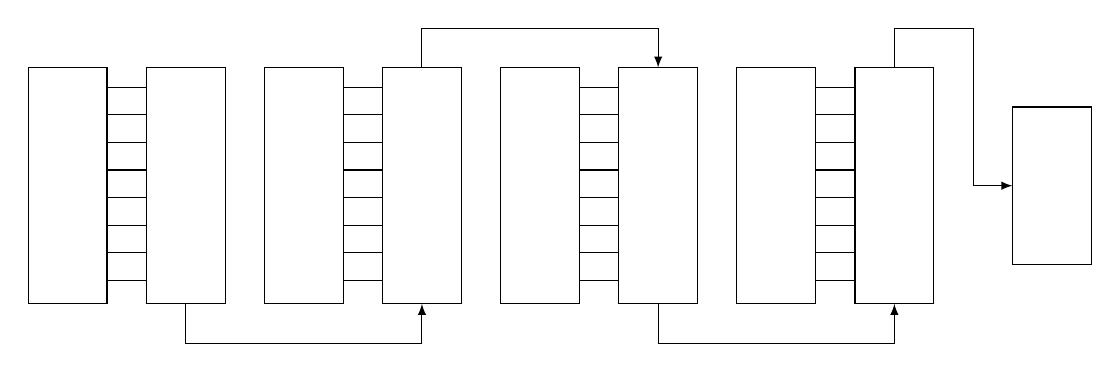
\begin{tikzpicture}[scale=.5]


%% serial shadowlatch
\draw  (28,1) rectangle (30,-5);
\draw (29,1) to (29,2) to (35,2)[>=latex,->]  to (35,1);
\draw (23,-5) to (23,-6) to (29,-6)[>=latex,->] to (29,-5);
\draw  (22,1) rectangle (24,-5);

\draw  (40,1) rectangle (42,-5);
\draw (41,1) to (41,2) to (43,2)[>=latex,->]  to (43,-2)  to (44,-2);
\draw (35,-5) to (35,-6) to (41,-6)[>=latex,->] to (41,-5);
\draw  (34,1) rectangle (36,-5);

\draw  (44,0) rectangle (46,-4);

\draw  (25,1) rectangle (27,-5);
\draw
(27,0.5)   to (28,0.5)
(27,-0.2) to (28,-0.2)
(27,-0.9)  to (28,-0.9)
(27,-1.6) to (28,-1.6)
(27,-2.3) to (28,-2.3)
(27,-3) to (28,-3)
(27,-3.7) to (28,-3.7)
(27,-4.4) to (28,-4.4);

\draw  (31,1) rectangle (33,-5);
\draw
(33,0.5)   to (34,0.5)
(33,-0.2) to (34,-0.2)
(33,-0.9)  to (34,-0.9)
(33,-1.6) to (34,-1.6)
(33,-2.3) to (34,-2.3)
(33,-3) to (34,-3)
(33,-3.7) to (34,-3.7)
(33,-4.4) to (34,-4.4);

\draw  (37,1) rectangle (39,-5);
\draw
(39,0.5)   to (40,0.5)
(39,-0.2) to (40,-0.2)
(39,-0.9)  to (40,-0.9)
(39,-1.6) to (40,-1.6)
(39,-2.3) to (40,-2.3)
(39,-3) to (40,-3)
(39,-3.7) to (40,-3.7)
(39,-4.4) to (40,-4.4);

\draw  (19,1) rectangle (21,-5);
\draw
(21,0.5)   to (22,0.5)
(21,-0.2) to (22,-0.2)
(21,-0.9)  to (22,-0.9)
(21,-1.6) to (22,-1.6)
(21,-2.3) to (22,-2.3)
(21,-3) to (22,-3)
(21,-3.7) to (22,-3.7)
(21,-4.4) to (22,-4.4);


\end{tikzpicture}
    \caption{Method of transporting data from TDCs to the FPGA using a one bit serial shift register without shadowlatches}
    \label{tkz:serial_no_shadow}
\end{figure}
